% NeurIPS 2026 Preprint -- Work in Progress
% Last updated: April 2026
%
% Build with: make paper (from project root)
% See paper/WORKFLOW.md for AI agent instructions

\documentclass{article}

% NeurIPS 2026 style (preprint mode)
\usepackage[preprint]{neurips_2026}

% Recommended packages
\usepackage[utf8]{inputenc}
\usepackage[T1]{fontenc}
\usepackage{microtype}
\usepackage{graphicx}
\usepackage{subcaption}
\usepackage{booktabs}
\usepackage{hyperref}
\usepackage{url}
\usepackage{amsmath,amssymb,mathtools,amsthm}
\usepackage[capitalize,noabbrev]{cleveref}
\usepackage{algorithm}
\usepackage{algorithmic}
\usepackage{enumitem}

% Path to figures (relative to paper/ directory, set via TEXINPUTS)
\graphicspath{{../figures/}}

%%%%%%%%%%%%%%%%%%%%%%%%%%%%%%%%
% THEOREMS AND MACROS
%%%%%%%%%%%%%%%%%%%%%%%%%%%%%%%%

\theoremstyle{plain}
\newtheorem{theorem}{Theorem}[section]
\newtheorem{proposition}[theorem]{Proposition}
\newtheorem{lemma}[theorem]{Lemma}
\newtheorem{corollary}[theorem]{Corollary}
\theoremstyle{definition}
\newtheorem{definition}[theorem]{Definition}
\newtheorem{assumption}[theorem]{Assumption}
\newtheorem{axiom}[theorem]{Axiom}
\theoremstyle{remark}
\newtheorem{remark}[theorem]{Remark}

\newcommand{\R}{\mathbb{R}}
\newcommand{\E}{\mathbb{E}}
\newcommand{\Q}{\hat{Q}}
\DeclareMathOperator{\KL}{KL}
\DeclareMathOperator{\Var}{Var}
\DeclareMathOperator{\Cov}{Cov}

\title{MALA-Guided Mirror Descent:\\Inference-Time Q-Guidance for Diffusion Policy RL\\[0.5em]\normalsize\textit{Preprint -- Work in Progress}}

\author{%
  Philip Nielsen \\
  Harvard University\\
  \texttt{pnielsen@seas.harvard.edu} \\
}

\begin{document}

\maketitle

\begin{abstract}
Policy improvement in reinforcement learning requires choosing an update rule, instantiating the targets implied by that rule and the current value estimate, and fitting a policy to those targets. Existing methods typically conflate these steps into a single optimization objective, limiting how accurately the intended update is realized. We separate them explicitly. We fix a class of policy-improvement rules given by $\alpha$-divergence mirror descent, which contains both standard mirror descent and maximum-entropy RL as special cases, and treat the induced update as a computational object that should be instantiated as accurately as possible before being amortized into a policy network. Concretely, we use MALA-corrected Q-guided sampling within a diffusion policy's reverse process to produce improved actions, which are then distilled into the policy through standard supervised learning. We further adapt the guidance strength online by modeling the distribution shift induced by the policy change itself, yielding a self-regulating update that balances exploitation against value-estimate staleness. This decomposition creates a natural axis along which additional computation improves the fidelity of the realized update rather than merely optimizing a fixed surrogate. On MuJoCo continuous-control benchmarks, our method achieves strong sample efficiency among model-free methods.
\end{abstract}

\section{Introduction}
\label{sec:intro}

Reinforcement learning for continuous control is typically implemented as an iterative policy improvement procedure. Given a current policy and a value estimate, the algorithm must determine how the policy should change and then realize that change within a parameterized policy class. In principle, much of the available improvement signal in RL lies in this step. In practice, however, existing methods often expose only a limited fraction of that signal, especially in continuous action spaces where the quality of the improvement step can strongly affect both sample efficiency and stability.

A useful way to view this problem is to separate three roles that are often conflated in modern RL algorithms. One must choose a policy improvement rule, instantiate the update-induced quantities implied by that rule and the current value estimate, and fit a policy network to those quantities. Depending on the method, these quantities may take the form of action samples, weights, denoising targets, or gradients rather than an explicit closed-form policy. The effectiveness of an RL algorithm depends on how well each of these pieces is handled. A principled update rule is not enough if the induced targets are instantiated inaccurately, and an expressive policy class is not enough if the targets presented to that policy are poor approximations of the desired improvement step.

Most existing methods do not make this separation explicit. Policy-gradient methods, including trust-region variants such as PPO \citep{schulman2017ppo} and TRPO \citep{schulman2015trust}, optimize surrogate objectives using local stochastic gradient information. These methods do not explicitly construct a target policy or target action distribution, so the realized update is tied to the locality and variance of the gradient signal and to whatever change the optimizer happens to induce in the policy network. KL-regularized actor-critic methods such as SAC \citep{haarnoja2018sac} go further by implicitly defining a target distribution over actions through a soft policy-improvement rule, but in practice they approximate this update inside a restricted policy class, typically Gaussian. This gives a tractable algorithm, but it also places a ceiling on how accurately the induced update can be represented and realized.

More recent methods based on expressive generative policies improve this picture only partially. By replacing simple parametric policies with diffusion \citep{ho2020denoising,song2021sde} or related policy classes, they make it easier to represent complex action distributions and therefore strengthen the projection step. However, the policy-improvement targets are still typically instantiated through approximate surrogates, for example weighted regression or score-matching objectives built from samples under the current policy \citep{ma2025soft}. In these approaches, additional computation is largely spent optimizing or estimating a surrogate within the chosen parameterization, rather than improving the fidelity of the induced policy update itself. Independent evidence for this difficulty comes from \citet{dong2025expo}, who find that directly backpropagating value gradients through expressive denoising chains causes instability, motivating alternative architectures that avoid this path entirely.

In this work, we separate these roles explicitly. We fix a class of policy-improvement rules given by $\alpha$-divergence mirror descent, which includes both standard mirror descent and maximum-entropy RL as special cases. We then treat the induced update as a computational object that should be instantiated as accurately as possible before being amortized into a policy network. The key insight is that policy improvement is fundamentally two problems: determining which actions should have been taken is hard, since even for bounded $\eta$ the tilted distribution $\pi \propto \pi_{\mathrm{old}} \exp(\eta Q)$ can be arbitrarily complex depending on the $Q$-landscape and requires iterative refinement to sample accurately, while fitting the generative model to those actions is comparatively easy, a standard supervised learning objective.

Concretely, we use an expressive diffusion policy together with inference-time MALA-corrected Q-guided sampling to produce improved actions at each denoising step, which are then distilled into the policy through unweighted behavioral cloning. This decomposition isolates the main sources of approximation error in policy improvement and creates a natural axis along which additional computation can improve the quality of the realized update, paralleling the test-time compute scaling paradigm that has proven effective in game-playing \citep{silver2017mastering} and language modeling \citep{snell2024scaling}, and recently validated for diffusion models through classical search \citep{zhang2025inference}. We further adapt the guidance strength $\eta$ online by modeling how the policy change alters the induced state distribution, yielding a self-regulating update analogous to trust-region methods \citep{kakade2002approximately,schulman2015trust}.

This separation provides several practical advantages: (i) the diffusion loss is simple and stable, with no effective-sample-size issues from importance weights; (ii) $\nabla_a Q$ is used directly at inference time, fully leveraging the learned value function; (iii) inference-time compute can be scaled independently of training by adjusting the number of MALA steps; and (iv) the guided actions stored in replay implicitly distill the inference-time improvement back into the base network, enabling iterative improvement in a loop structurally analogous to AlphaGo Zero \citep{silver2017mastering}, which uses MCTS to produce actions better than the policy network alone, then trains the network to match. Empirically, we show that this combination yields strong sample efficiency on standard continuous-control benchmarks among model-free methods while maintaining stable training.

\section{Related Work}
\label{sec:related}

\subsection{Diffusion policies for reinforcement learning}

Diffusion models have been adopted as policy classes in both offline and online RL.
In offline RL, Diffuser \citep{janner2022diffuser} denoises entire state-action trajectories conditioned on desired returns, while DiffusionQL \citep{lu2024diffusionql}, IDQL \citep{hansen2023idql}, and \citet{wang2023diffusion} use diffusion models as expressive policy classes for continuous control.
\citet{chi2023diffusion} apply diffusion policies to imitation learning for robotic manipulation.

In online RL, the central challenge is how to incorporate the learned value function into the diffusion policy.
DPMD \citep{ma2025soft} implements the mirror descent tilt at training time by reweighting the denoising loss with exponentiated $Q$-values, a form of advantage-weighted regression applied to diffusion.
SDAC \citep{ma2025soft} targets the maximum-entropy policy through a related reweighting.
QSM \citep{psenka2024qsm} trains the diffusion score to match $\nabla_a Q / \alpha$ directly, and DIPO \citep{yang2023dipo} modifies replay actions using $\nabla_a Q$ before training.
All of these methods incorporate the value function at training time, either through loss reweighting or gradient-based modifications to the training data or objective.

A separate line of work avoids direct value optimization of the diffusion policy altogether.
EXPO \citep{dong2025expo} trains the base diffusion policy with imitation learning and introduces a lightweight Gaussian edit policy that nudges base-policy actions toward higher $Q$-values, selecting the best action on the fly.
\citet{dong2025expo} report that training-time gradient-based methods such as QSM collapse during online fine-tuning, providing independent evidence for the instability of backpropagating value gradients through denoising chains.
CFGRL \citep{frans2025cfgrl} derives a formal connection between classifier-free guidance strength and policy improvement, but operates only in the offline setting.
MGMD shares the principle of avoiding training-time value optimization of the diffusion policy, but differs from EXPO in using gradient-based MCMC within the diffusion process itself rather than a separate edit network.

\subsection{Inference-time guidance and MCMC for diffusion models}

Guidance methods modify the reverse diffusion process to steer samples toward regions of high reward or likelihood under an external objective.
Classifier guidance \citep{dhariwal2021beatgans} adds the gradient of a noise-level-dependent classifier to the score, while classifier-free guidance \citep{ho2022classifierfree} interpolates between conditional and unconditional score predictions without requiring a separate classifier.
Training-free guidance (TFG) \citep{ye2024tfg,bansal2023universal} generalizes this idea to arbitrary differentiable objectives by evaluating them on clean-action estimates obtained via Tweedie's formula.
However, the TFG-guided reverse process does not correspond to the time reversal of any well-defined forward diffusion, so it does not guarantee sampling from the correctly tilted distribution.

MCMC corrections address this gap.
\citet{du2023reduce_reuse_recycle} show how to combine energy-based objectives with a base diffusion model by applying Metropolis-Hastings corrections at each noise level, producing samples that asymptotically follow the desired tilted distribution.
MGMD builds directly on this framework, specializing the energy term to $Q$-guidance for online RL and using MALA with adaptive per-level step sizes as the corrector.

Recent work has studied inference-time compute scaling for diffusion models more broadly.
\citet{zhang2025inference} combine annealed Langevin MCMC with breadth-first and depth-first tree search, validating gradient-based MCMC as a principled approach to inference-time scaling across planning, offline RL, and image generation.
\citet{ma2025scaling} frame inference-time scaling as a search problem over noise candidates evaluated by verifiers, demonstrating substantial quality gains on image generation benchmarks.
\citet{su2025navigating} study the exploration-exploitation tradeoff inherent in particle-based inference-time methods.
MGMD builds on the same Langevin dynamics framework as \citet{zhang2025inference} but adds Metropolis-Hastings acceptance corrections for asymptotically exact sampling, applies it to online RL with adaptive guidance strength, and operates on a single action particle rather than maintaining a population.

\subsection{Policy extraction from value functions}

A central challenge in RL with expressive policy classes is how to convert a learned $Q$-function into an improved policy.
\citet{park2024bottleneck} show that the choice of policy extraction method is often more impactful than the quality of value learning itself, with gradient-based extraction (DDPG+BC) consistently outperforming both advantage-weighted regression (AWR) and rejection sampling.

Existing extraction methods for diffusion policies fall into three categories.
Weighted behavioral cloning, used by DPMD \citep{ma2025soft}, reweights the denoising loss by exponentiated $Q$-values. This is a form of AWR applied to diffusion and can suffer from effective sample size collapse when $Q$-values concentrate on a few transitions.
Rejection sampling, such as best-of-$N$ selection \citep{ma2025soft,espinosa2025evor}, draws multiple action candidates and selects the highest-$Q$ one. This uses no gradient information and scales poorly with action dimensionality: in an environment composed of $k$ independent subtasks, rejection sampling requires $\Omega((1/p)^k)$ candidates to find a jointly good action, while gradient-based methods decompose across subtasks and scale linearly.
Distillation approaches such as FQL \citep{park2025fql} compress a multi-step flow policy into a one-step model that can be optimized directly with $\nabla_a Q$, and SORL \citep{espinosa2025sorl} uses shortcut models with best-of-$N$ selection to enable inference-time compute scaling.

MGMD performs gradient-based extraction at inference time via MALA, combining the effectiveness of gradient-based methods identified by \citet{park2024bottleneck} with the training stability of unweighted behavioral cloning. Unlike distillation approaches that require architectural changes, MGMD operates within the standard diffusion sampling process.

\subsection{Inference-time compute scaling and amortization}

A policy network is an amortized optimizer: it maps states to actions using shared weights and cannot perfectly optimize $Q$ for each individual state. \citet{marino2021iterative} formalize this as an amortization gap and show that iterative refinement at inference time can close it. \citet{chalumeau2025breaking} provide large-scale evidence that inference strategies can break through the performance ceilings of well-trained RL policies, even when additional training provides diminishing returns.

This principle has a longer history in discrete domains. AlphaGo Zero \citep{silver2017mastering} uses MCTS to produce actions better than the policy network alone, then trains the network to match the MCTS output. The network serves as an amortized approximation to the inference-time-improved policy, and each training cycle closes the amortization gap. MGMD's MALA-plus-distillation loop is structurally identical: guided sampling produces improved actions, and unweighted BC distills them back into the base policy. More recently, test-time compute scaling has emerged as a powerful paradigm in language modeling \citep{snell2024scaling}, where additional inference-time computation yields gains that complement or exceed those from scaling model parameters.

MGMD extends this paradigm to online continuous-control RL with diffusion policies. The distillation loop ensures that inference-time improvements are not discarded but accumulate in the base policy across training iterations.

\subsection{Adaptive step sizes and trust regions}

The guidance strength $\eta$ in MGMD controls how aggressively the sampler tilts toward high-$Q$ actions. Setting this parameter is closely related to the step-size problem in policy optimization.
Conservative Policy Iteration \citep{kakade2002approximately} trades off a first-order improvement term against a second-order distribution-shift penalty via a mixing rate, establishing the structural template that stronger updates are not always better because they increase the staleness of the value estimates used to compute the update.
TRPO \citep{schulman2015trust} operationalizes this by constraining $\KL(\pi_{\mathrm{new}} \| \pi_{\mathrm{old}})$ to the region where the surrogate objective remains reliable.
SAC \citep{haarnoja2018sac} tunes its entropy temperature adaptively via a Lagrangian on target entropy, but does not model how the policy change itself alters the value landscape.

MGMD's adaptive $\eta$ builds on this line of work. A KL budget rule provides scale invariance by normalizing $\eta$ by $1/\sqrt{\Var(A)}$, ensuring the update is invariant to reward rescaling. A tighter rule derived from a second-order expansion of the true policy improvement $\Delta V$ accounts for the covariance between current advantages and downstream advantage variance, yielding an optimal $\eta^*$ at which the marginal benefit of stronger tilting exactly equals the marginal cost of $Q$-value staleness (see \cref{sec:adaptive-eta}).

\section{Background}
\label{sec:background}

\subsection{Reinforcement learning and mirror descent}
\label{sec:rl-background}

We consider an infinite-horizon MDP $\mathcal{M} = (\mathcal{S}, \mathcal{A}, P, R, \gamma)$ with continuous action space $\mathcal{A} \subseteq \mathbb{R}^d$, transition kernel $P$, reward function $R$, and discount factor $\gamma \in [0,1)$.
A policy $\pi: \mathcal{S} \to \Delta(\mathcal{A})$ maps states to distributions over actions.
The goal is to find a policy maximizing $J(\pi) = \E_\pi[\sum_{t=0}^\infty \gamma^t R(s_t, a_t)]$, where the state-action value $Q^\pi(s,a) = \E_\pi[\sum_{t=0}^\infty \gamma^t R(s_t,a_t) \mid s_0{=}s, a_0{=}a]$ and the advantage $A^\pi(s,a) = Q^\pi(s,a) - V^\pi(s)$ characterize the expected return.

In maximum-entropy RL \citep{haarnoja2018sac}, the objective is augmented with an entropy bonus, and the optimal policy update takes the form of a mirror descent step:
\begin{equation}
  \pi_{\mathrm{new}}(a\mid s) \propto \pi_\mathrm{old}(a\mid s) \exp\{\eta Q(s,a)\},
  \label{eq:md-tilt}
\end{equation}
where $\eta > 0$ controls the step size.
For Gaussian policies, this update can be approximately implemented via reparameterized policy gradients \citep{haarnoja2018sac}.

\paragraph{Step size selection.}
Imposing a KL budget $\Delta$ on the per-state divergence $\KL(\pi_{\mathrm{new}}(\cdot|s) \| \pi_{\mathrm{old}}(\cdot|s)) \le \Delta$ and expanding to second order yields the scale-invariant rule
\begin{equation}
  \eta = \sqrt{\frac{2\Delta}{\E_{s}[\Var_{\pi}(Q(s,\cdot))]}},
  \label{eq:kl-budget-eta}
\end{equation}
which normalizes the step size by the variance of $Q$-values under the current policy.
In \cref{sec:adaptive-eta}, we derive a tighter rule that accounts for the distribution shift induced by the policy change itself.

\subsection{Diffusion models as policies}
\label{sec:diffusion-background}

Diffusion models \citep{ho2020denoising,song2021sde} generate samples through an iterative denoising process.
A fixed forward process corrupts a clean action $a_0$ to a noisy version $a_t = \sqrt{\bar{\alpha}_t}\, a_0 + \sqrt{1-\bar{\alpha}_t}\, \epsilon$, where $\epsilon \sim \mathcal{N}(0,I)$ and $\bar{\alpha}_t = \prod_{i=1}^t (1-\beta_i)$ is the cumulative noise schedule.
A neural network $\epsilon_\theta$ is trained to reverse this process via the denoising score matching objective:
\begin{equation}
  \mathcal{L}_{\text{DSM}} = \E_{a_0, \epsilon, t}\bigl[\|\epsilon_\theta(a_t, s, t) - \epsilon\|^2\bigr].
  \label{eq:dsm}
\end{equation}
The optimal noise predictor satisfies $\epsilon_\theta^*(a_t, s, t) = -\sqrt{1{-}\bar{\alpha}_t}\, \nabla_{a_t} \log p_t(a_t \mid s)$, so that learning to denoise is equivalent to learning the score \citep{ho2020denoising}.

When the model is parameterized in energy-based form, a scalar energy $E_\theta(a_t, s, t)$ is output and the score is obtained by automatic differentiation: $\nabla_{a_t} \log p_\theta(a_t \mid s, t) = -\nabla_{a_t} E_\theta(a_t, s, t)$.
Training proceeds by the same denoising objective \cref{eq:dsm}, but the energy-based form additionally enables computing Metropolis-Hastings acceptance probabilities (see \cref{sec:mala}).

At inference time, actions are generated by sampling $a_T \sim \mathcal{N}(0,I)$ and iteratively applying the learned denoising process to produce $a_0$.
The clean-action estimate at any noise level $t$ can be obtained via Tweedie's formula:
\begin{equation}
  \hat{a}_0(a_t) = \frac{a_t - \sqrt{1-\bar{\alpha}_t}\, \epsilon_\theta(a_t, s, t)}{\sqrt{\bar{\alpha}_t}}.
  \label{eq:tweedie}
\end{equation}

\subsection{Policy improvement for diffusion policies}
\label{sec:policy-improvement-bg}

Given a diffusion policy $\pi_\theta(a \mid s)$ and a learned $Q$-function, the challenge is to implement the mirror-descent update \cref{eq:md-tilt}: sampling from $\pi_{\mathrm{new}}(a\mid s) \propto \pi_\mathrm{old}(a\mid s) \exp\{\eta Q(s,a)\}$.
In online RL, this target distribution depends on the current $Q$-function, which changes with each training iteration.

\paragraph{Weighted behavioral cloning.}
DPMD \citep{ma2025soft} implements the mirror-descent update at training time by reweighting the denoising loss:
\begin{equation}
  \mathcal{L}_{\text{DPMD}} = \E\big[ w(s,a) \; \| \epsilon_\theta(a_t,s,t) - \epsilon \|^2 \big],
\end{equation}
where $w(s,a)$ is derived from a standardized, exponentiated version of $Q(s,a)$.
At inference time, DPMD draws $N$ action candidates and selects the one with the highest $Q$-value.

\paragraph{Training-free guidance.}
An alternative is to modify the sampling process.
Training-free guidance (TFG) \citep{ye2024tfg,bansal2023universal} evaluates the objective on the clean action estimate \cref{eq:tweedie} and modifies the noise prediction:
\begin{equation}
  \epsilon_{\text{guided}} = \epsilon_\theta - \lambda_t \sqrt{1-\bar{\alpha}_t}\, \nabla_{a_t} Q(s, \hat{a}_0(a_t)),
  \label{eq:tfg-update}
\end{equation}
where $\lambda_t$ is a noise-level-dependent guidance weight.
However, the TFG-guided reverse process does not correspond to the time reversal of any well-defined forward diffusion, so it does not guarantee sampling from the tilted distribution \cref{eq:md-tilt}.

\section{Method}
\label{sec:methods}

MGMD separates policy improvement into two stages: a hard stage that uses inference-time sampling to produce actions from the mirror-descent tilt \cref{eq:md-tilt}, and an easy stage that fits the diffusion policy to those actions via unweighted behavioral cloning.
At training time, the policy is updated by minimizing the standard denoising objective \cref{eq:dsm} with uniform weights on replay buffer actions, which, in the online setting, are the guided actions stored during environment interaction.
Twin $Q$-networks are trained via off-policy TD learning.
All $Q$-based policy improvement occurs at inference time.

\subsection{Why guidance requires MCMC corrections}
\label{sec:why-mcmc}

To understand why TFG alone is insufficient, consider the target tilted distribution $\tilde{p}_0(a_0 \mid s) \propto p_0(a_0 \mid s) \exp\{\eta Q(s, a_0)\}$.
For standard DDPM sampling to produce exact samples from $\tilde{p}_0$, the reverse process would need to follow the score of the noisy tilted marginals:
\begin{equation}
  \tilde{p}_t(a_t \mid s) = \int p_{t|0}(a_t \mid a_0)\, \tilde{p}_0(a_0 \mid s)\, da_0.
  \label{eq:tilted-marginal}
\end{equation}
While the score decomposes additively at $t=0$ ($\nabla_{a_0} \log \tilde{p}_0 = \nabla_{a_0} \log p_0 + \eta \nabla_{a_0} Q$), this does not hold for $t > 0$:
\begin{equation}
  \nabla_{a_t} \log \tilde{p}_t(a_t) \neq \nabla_{a_t} \log p_t(a_t) + \eta \nabla_{a_t} Q(s, \hat{a}_0(a_t)).
  \label{eq:score-mismatch}
\end{equation}
The TFG update \cref{eq:tfg-update} therefore does not produce exact samples from the tilted distribution.

\paragraph{Energy-based target sequence.}
Following \citet{du2023reduce_reuse_recycle}, we instead interpret the guided sampler as targeting a sequence of energy-based distributions:
\begin{equation}
  q_t(a_t \mid s) \propto \exp\bigl\{-E_t(a_t, s)\bigr\}, \qquad
  E_t(a_t, s) = E_\theta(a_t, s, t) - \lambda_t Q(s, \hat{a}_0(a_t)),
  \label{eq:energy-sequence}
\end{equation}
where $\lambda_t$ is a noise-level-dependent guidance weight.
These distributions interpolate smoothly from a nearly Gaussian distribution at $t=T$ (where $\hat{a}_0$ is a poor estimate and guidance has little effect) to the desired tilted policy at $t=0$ (where $\hat{a}_0 \approx a_0$).
However, even if samples at noise level $t$ follow $q_t$, a single guided DDPM step does not guarantee that the resulting samples follow $q_{t-1}$, because the sequence $\{q_t\}$ does not arise from any forward diffusion process.
MCMC corrections at each noise level address this sampling gap.

\paragraph{Why gradient-based corrections scale better than rejection sampling.}
Consider an environment composed of $k$ independent copies of a base task, so that $a = (a^1, \ldots, a^k) \in \mathbb{R}^{k d_0}$ and $Q(s,a) = \sum_{i=1}^k Q_i(s^i, a^i)$.
For rejection sampling (best-of-$N$), a good action must be good in all $k$ subspaces simultaneously.
If good actions in each subspace have probability $p$ under the base policy, a jointly good action has probability $p^k$, requiring $N = \Omega((1/p)^k)$ candidates.
For MALA, the gradient $\nabla_a Q = (\nabla_{a^1} Q_1, \ldots, \nabla_{a^k} Q_k)$ decomposes across subspaces, so each Langevin step independently moves toward good actions in each copy.
The cost scales linearly, not exponentially, with dimension.

\subsection{MALA-corrected Q-guidance}
\label{sec:mala}

We use the Metropolis-Adjusted Langevin Algorithm (MALA) to correct the guided sampler at each noise level.
MALA combines gradient-based proposals with Metropolis-Hastings (MH) acceptance, providing asymptotic guarantees on the sampling distribution.

\paragraph{Composite energy.}
At each diffusion level $t$, we define the total energy combining the learned prior with the $Q$-function:
\begin{equation}
  E_t^{\text{total}}(a_t, s) = E_\theta(a_t, s, t) - \lambda_t \, Q_\phi(s, \hat{a}_0(a_t)),
  \label{eq:total-energy}
\end{equation}
where $\hat{a}_0(a_t)$ is the Tweedie estimate \cref{eq:tweedie} clipped to $[-r, r]$, $Q_\phi$ is an aggregation of the twin critics (mean of $Q_{\phi_1}, Q_{\phi_2}$), and $\lambda_t$ is a noise-level-dependent guidance weight that controls how the global guidance strength $\eta$ is distributed across diffusion levels.
The corresponding Boltzmann distribution $q_t(a_t) \propto \exp\{-E_t^{\text{total}}(a_t, s)\}$ is our target at level $t$.

MH corrections require evaluating the energy $E_t^{\text{total}}$ (not just its gradient), which is why the diffusion model must be parameterized in energy-based form.

\paragraph{MALA corrector.}
At each diffusion level, we apply $K$ MALA corrector steps targeting $q_t$.
A single step proposes:
\begin{equation}
  a_t' = a_t - \tilde{\eta}_t \nabla_{a_t} E_t^{\text{total}}(a_t, s) + \sqrt{2\tilde{\eta}_t}\, z, \quad z \sim \mathcal{N}(0, I),
  \label{eq:mala-proposal}
\end{equation}
where $\tilde{\eta}_t$ is the MALA step size at level $t$ (distinct from the guidance strength $\eta$).
The proposal is accepted with probability
\begin{equation}
  \alpha = \min\Bigl(1, \frac{q_t(a_t') \, \mathcal{T}(a_t \mid a_t')}{q_t(a_t) \, \mathcal{T}(a_t' \mid a_t)}\Bigr),
  \label{eq:mh-accept}
\end{equation}
where $\mathcal{T}(a' \mid a) = \mathcal{N}(a' ; a - \tilde{\eta}_t \nabla E_t^{\text{total}}, 2\tilde{\eta}_t I)$ is the Langevin proposal kernel.
The gradient $\nabla_{a_t} E_t^{\text{total}}$ incorporates $\nabla_a Q$ via the chain rule through the Tweedie estimate, directly leveraging the learned value function.

\paragraph{Adaptive MALA step sizes.}
Following \citet{RobertsTweedie1996MALA}, the optimal acceptance rate for MALA in high dimensions is approximately $0.574$.
We parameterize the MALA step size as $\tilde{\eta}_t = \sigma_t \cdot \exp(\ell_t)$, where $\sigma_t = \beta_t$ is the noise schedule at level $t$ and $\ell_t$ is a learnable log-scale factor.
A Robbins-Monro update adapts $\ell_t$ after each MALA step:
\begin{equation}
  \ell_t \leftarrow \ell_t + \alpha_{\text{adapt}} \bigl(\text{acc\_rate}_t - \alpha^*\bigr),
  \label{eq:eta-adapt}
\end{equation}
where $\alpha^* = 0.574$ is the target acceptance rate and $\alpha_{\text{adapt}}$ is the adaptation rate.
Per-level adaptation is essential: the energy landscape is smooth at high noise levels (requiring larger steps) and sharp at low noise levels (requiring smaller steps).

\paragraph{Guided predictor.}
Between MALA corrector phases, a DDIM predictor step transitions from noise level $t$ to $t{-}1$.
The predictor incorporates $Q$-guidance by modifying the noise prediction:
\begin{equation}
  \epsilon_{\text{pred}} = \epsilon_\theta(a_t, s, t) - \lambda_t \sqrt{1{-}\bar{\alpha}_t} \, \nabla_{a_t} Q_\phi(s, \hat{a}_0(a_t)),
  \label{eq:guided-predictor}
\end{equation}
and applying the deterministic DDIM update with this modified prediction.

\paragraph{Predictor-corrector structure.}
The full MGMD sampler interleaves predictor and corrector steps.
Starting from $a_T \sim \mathcal{N}(0, I)$, for each level $t = T{-}1, \ldots, 0$: (1) apply $K$ MALA corrector steps targeting $q_t$, adapting $\tilde{\eta}_t$; then (2) apply the guided DDIM predictor to obtain $a_{t-1}$.
This predictor-corrector structure, following \citet{du2023reduce_reuse_recycle}, ensures samples approximately follow the sequence of tilted distributions while the predictor provides efficient transitions between noise levels.
The complete sampling procedure is given in \cref{alg:tilted-sampling}.

\subsection{Training}
\label{sec:training}

The training procedure decouples value learning from policy fitting.

\paragraph{Critic.}
Twin $Q$-networks $Q_{\phi_1}, Q_{\phi_2}$ are trained via standard off-policy TD learning.
For TD target computation, next-state actions are drawn from the guided sampler (\cref{alg:tilted-sampling}), and the bootstrap value uses the minimum of the twin critics: $y = r + \gamma \min(Q_{\phi_1'}(s', a'), Q_{\phi_2'}(s', a'))$, where $\phi_1', \phi_2'$ are slowly-updated target network parameters.
Using guided actions for TD targets means the critic evaluates the implicit policy defined by the inference-time procedure rather than the amortized base policy.

\paragraph{Policy.}
The diffusion policy is trained by minimizing the standard denoising objective \cref{eq:dsm} with uniform weights on replay buffer actions.
Because the replay buffer stores the guided actions produced during environment interaction, the policy is effectively distilled from the inference-time-improved action distribution.
This avoids the effective-sample-size issues of $Q$-reweighted denoising losses: all training samples contribute equally, while the quality of the targets is determined by the MALA sampling procedure rather than by importance weights.

\paragraph{Critic normalization.}
When adaptive guidance strength is used (\cref{sec:adaptive-eta}), the $Q$-values used for guidance are normalized by a running estimate of the advantage standard deviation: the guidance signal becomes $A(s,a) / \hat{\sigma}_A$, where $A(s,a) = Q(s,a) - V(s)$ and $\hat{\sigma}_A$ is maintained as an exponential moving average of $\sqrt{\E[A^2]}$.
This normalization ensures that the guidance magnitude is invariant to the scale of returns.

\subsection{Adaptive guidance strength}
\label{sec:adaptive-eta}

The guidance strength $\eta$ in \cref{eq:total-energy} controls how aggressively the sampler tilts toward high-$Q$ actions.
Rather than treating $\eta$ as a fixed hyperparameter, we derive two adaptive rules by analyzing the policy improvement $\Delta V(s;\eta) \coloneqq V^{\pi_\eta}(s) - V^\pi(s)$ as a function of $\eta$.

\paragraph{KL budget rule.}
The KL budget rule \cref{eq:kl-budget-eta} sets $\eta \propto 1/\sqrt{\Var(Q)}$, ensuring scale invariance: the update is unchanged if all rewards are multiplied by a constant. This serves as a baseline and ceiling for the guidance strength.

\paragraph{Distribution-shift-aware rule.}
The KL budget rule does not account for the fact that after the policy changes, the $Q$-values used to compute the tilt become stale.
We expand $\Delta V$ to second order in $\eta$, substituting $Q^{\pi_\eta} = Q^\pi + \gamma \E_{s'|s,a}[\Delta V(s';\eta)]$ to model the downstream effect of the policy change.
Averaging over the state distribution yields
\begin{equation}
  \E_{s}[\Delta V(s;\eta)] \approx \eta\, v^\pi + \eta^2\!\left(\gamma c^\pi + \tfrac{1}{2}\kappa_3^\pi\right),
  \label{eq:delta-v-expansion}
\end{equation}
where $v^\pi = \E_s[\Var_\pi(A)]$ is the expected advantage variance, $\kappa_3^\pi = \E_s[\E_\pi[A^3]]$ is the third moment, and $c^\pi = \E_s[\Cov_\pi(\E_{s'}[\Var_{\pi'}(A')],\, A)]$ captures the covariance between current advantages and the downstream advantage variance.
Optimizing over $\eta$ gives
\begin{equation}
  \boxed{\;\eta^* = -\frac{v^\pi}{2\gamma c^\pi + \kappa_3^\pi} = -\frac{1}{\sqrt{v^\pi}\, s^\pi}\;}
  \label{eq:eta-star}
\end{equation}
where $s^\pi = (2\gamma c^\pi + \kappa_3^\pi) / (v^\pi)^{3/2}$ is a dimensionless shape statistic.
The guidance strength is set to $\eta = \min(\eta^*, \eta_{\text{KL}})$ when the shape $s^\pi < 0$ (indicating that the quadratic model predicts a finite optimum), and falls back to the KL budget ceiling $\eta_{\text{KL}}$ otherwise.
The full derivation and practical EMA estimation procedure are given in \cref{app:adaptive-eta}.

\paragraph{Connection to trust region methods.}
This second-order expansion mirrors the structure of classical policy improvement bounds.
In CPI \citep{kakade2002approximately}, a mixing rate trades off first-order improvement against second-order distribution shift; in TRPO \citep{schulman2015trust}, a trust region constrains the step to where the surrogate remains reliable.
Our $\eta^*$ plays the same role: it is the guidance strength at which the marginal benefit of stronger tilting exactly equals the marginal cost of $Q$-value staleness.
Beyond $\eta^*$, additional tilting is counterproductive, so the method self-regulates against over-exploitation.

\subsection{Algorithm summary}
\label{sec:algorithm}

The overall MGMD training loop is given in \cref{alg:mgmd} and the tilted sampling subroutine in \cref{alg:tilted-sampling}.
Full hyperparameter settings are given in \cref{app:hyperparams}.

\begin{algorithm}[t]
\caption{MGMD: MALA-Guided Mirror Descent}
\label{alg:mgmd}
\begin{algorithmic}[1]
\STATE \textbf{Input:} Environment $\mathcal{M}$, replay buffer $\mathcal{D}$, guidance strength $\eta$ (fixed or adaptive, \cref{sec:adaptive-eta})
\STATE Initialize diffusion policy $\pi_\theta$ (energy-based), twin critics $Q_{\phi_1}, Q_{\phi_2}$, target networks $Q_{\phi_1'}, Q_{\phi_2'}$, MALA log-scales $\{\ell_t\}_{t=0}^{T-1}$
\FOR{each environment step}
  \STATE Observe state $s$
  \STATE $a \leftarrow \textsc{TiltedSample}(s, \pi_\theta, Q_\phi, \eta, \{\ell_t\})$ \hfill $\triangleright$ \cref{alg:tilted-sampling}
  \STATE Execute $a$, observe $r, s'$; store $(s, a, r, s')$ in $\mathcal{D}$
  \FOR{$j = 1, \ldots, G$ gradient steps}
    \STATE Sample minibatch $\{(s_i, a_i, r_i, s_i')\}$ from $\mathcal{D}$
    \STATE \textbf{Critic update:}
    \STATE \quad $a_i' \leftarrow \textsc{TiltedSample}(s_i', \pi_\theta, Q_\phi, \eta, \{\ell_t\})$
    \STATE \quad $y_i \leftarrow r_i + \gamma \min(Q_{\phi_1'}(s_i', a_i'), Q_{\phi_2'}(s_i', a_i'))$
    \STATE \quad Update $\phi_1, \phi_2$ to minimize $\sum_i (Q_{\phi_k}(s_i, a_i) - y_i)^2$
    \STATE \quad Polyak-update targets: $\phi_k' \leftarrow \tau \phi_k + (1{-}\tau)\phi_k'$
    \STATE \textbf{Policy update:}
    \STATE \quad Update $\theta$ to minimize $\mathcal{L}_{\text{DSM}}$ (\cref{eq:dsm}) with uniform weights on $\{a_i\}$
    \STATE \textbf{Adaptive $\eta$} (if enabled): update EMAs and recompute $\eta$ (\cref{sec:adaptive-eta})
  \ENDFOR
\ENDFOR
\end{algorithmic}
\end{algorithm}

\begin{algorithm}[t]
\caption{TiltedSample: MALA-Corrected Q-Guided Diffusion Sampling}
\label{alg:tilted-sampling}
\begin{algorithmic}[1]
\STATE \textbf{Input:} State $s$, policy $\pi_\theta$, critic $Q_\phi$, guidance strength $\eta$, MALA log-scales $\{\ell_t\}$
\STATE \textbf{Parameters:} Diffusion steps $T$, noise schedule $\{\beta_t, \bar{\alpha}_t\}$, guidance schedule $\{\lambda_t\}$, MALA steps $K$, clip radius $r$, adaptation rate $\alpha_{\text{adapt}}$, target acceptance $\alpha^*$
\STATE Sample $a_T \sim \mathcal{N}(0, I)$
\FOR{$t = T{-}1, \ldots, 0$}
  \FOR{$k = 1, \ldots, K$}
    \STATE Compute Tweedie estimate: $\hat{a}_0 \leftarrow \text{clip}\!\left(\frac{a_t - \sqrt{1-\bar{\alpha}_t}\,\epsilon_\theta(a_t, s, t)}{\sqrt{\bar{\alpha}_t}},\; -r,\; r\right)$
    \STATE Compute energy: $E_t \leftarrow E_\theta(a_t, s, t) - \lambda_t \, Q_\phi(s, \hat{a}_0)$ \hfill $\triangleright$ Eq.~\ref{eq:total-energy}
    \STATE Compute gradient: $g \leftarrow \nabla_{a_t} E_t$
    \STATE Set step size: $\tilde{\eta}_t \leftarrow \text{clip}(\beta_t \cdot \exp(\ell_t),\; \tilde{\eta}_{\min},\; \tilde{\eta}_{\max})$
    \STATE Propose: $a_t' \leftarrow a_t - \tilde{\eta}_t \, g + \sqrt{2\tilde{\eta}_t}\, z$, \quad $z \sim \mathcal{N}(0,I)$ \hfill $\triangleright$ Eq.~\ref{eq:mala-proposal}
    \STATE Compute $E_t', g'$ at $a_t'$ (same as lines 6--8)
    \STATE MH accept/reject: $\alpha \leftarrow \min\!\big(1,\; \exp\!\big[(E_t {-} E_t') + \frac{\|a_t - (a_t' - \tilde{\eta}_t g')\|^2 - \|a_t' - (a_t - \tilde{\eta}_t g)\|^2}{4\tilde{\eta}_t}\big]\big)$
    \STATE Accept $a_t \leftarrow a_t'$ with probability $\alpha$, else keep $a_t$
    \STATE Adapt: $\ell_t \leftarrow \text{clip}(\ell_t + \alpha_{\text{adapt}}(\alpha - \alpha^*),\; \ell_{\min},\; \ell_{\max})$ \hfill $\triangleright$ Eq.~\ref{eq:eta-adapt}
  \ENDFOR
  \STATE \textbf{Guided predictor} (DDIM) from level $t$ to $t{-}1$: \hfill $\triangleright$ Eq.~\ref{eq:guided-predictor}
  \STATE \quad $\epsilon_{\text{pred}} \leftarrow \epsilon_\theta(a_t, s, t) - \lambda_t \sqrt{1{-}\bar{\alpha}_t} \, \nabla_{a_t} Q_\phi(s, \hat{a}_0(a_t))$
  \STATE \quad $a_{t-1} \leftarrow \text{DDIM}(a_t, \epsilon_{\text{pred}}, t)$
\ENDFOR
\STATE \textbf{Return} $a_0$
\end{algorithmic}
\end{algorithm}

\section{Experiments}
\label{sec:experiments}

We evaluate MGMD on MuJoCo continuous-control benchmarks from OpenAI Gym.
All experiments train for $10^6$ environment steps with five random seeds using five parallel environments for data collection.
We report the mean final evaluation return with 90\% confidence intervals computed via the $t$-distribution across seeds.

\begin{figure}[t]
  \centering
  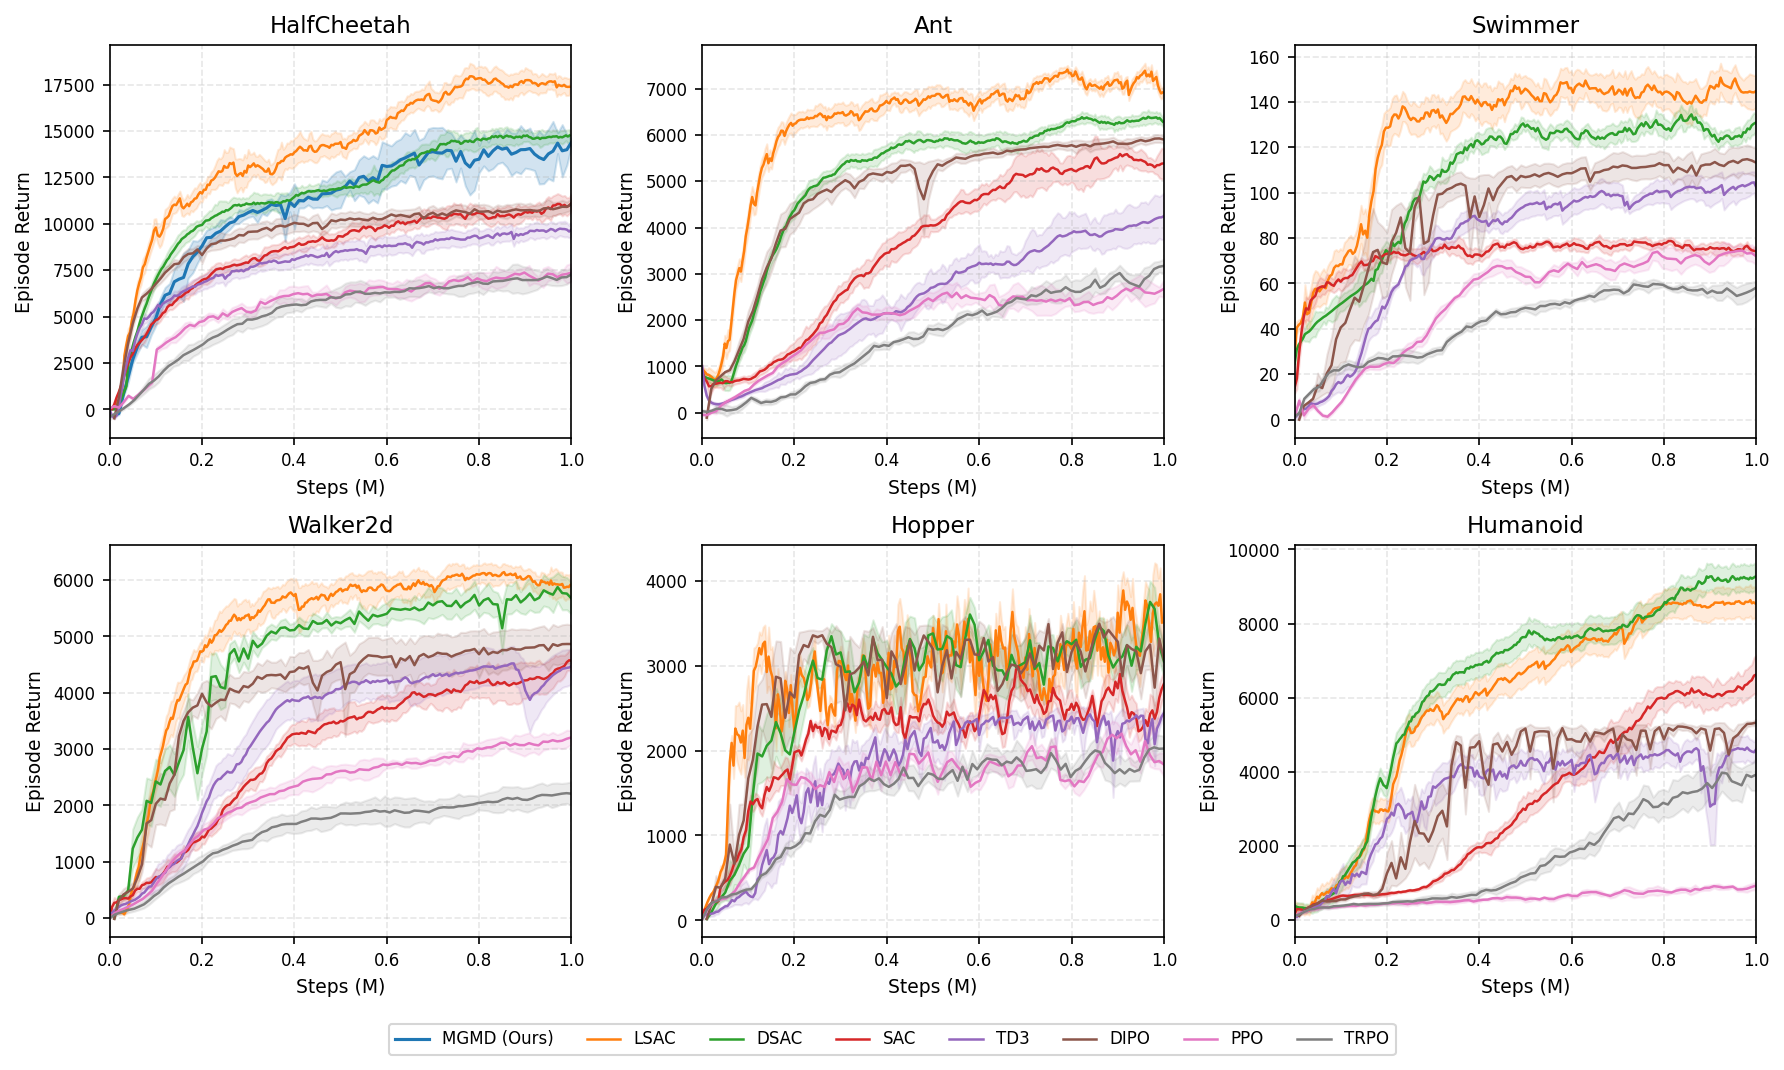
\includegraphics[width=\textwidth]{model_free_training_curves_all_envs.png}
  \caption{Training curves across six MuJoCo environments over $10^6$ steps. MGMD uses 10 seeds on HalfCheetah and 1 seed elsewhere; baselines use 10 seeds. Shaded regions show 90\% CI via the $t$-distribution.}
  \label{fig:training-curves}
  \vskip -0.1in
\end{figure}

\subsection{Setup}
\label{sec:setup}

\paragraph{Architecture.}
The diffusion policy and critic use three-layer MLPs with 256 hidden units and Mish activations \citep{misra2019mish}.
The policy uses an energy-based parameterization where the network outputs a scalar energy and the score is computed via automatic differentiation.
The critic consists of twin $Q$-networks trained with Huber loss.

\paragraph{Baselines.}
We compare against:
\begin{itemize}[nosep]
  \item \textbf{SAC} \citep{haarnoja2018sac}: Soft Actor-Critic with Gaussian policies.
  \item \textbf{TD3}: Twin delayed DDPG.
  \item \textbf{DIPO} \citep{yang2023dipo}: Diffusion policy with gradient-based action modification.
  \item \textbf{RedQ}: Randomized ensemble double Q-learning.
  \item \textbf{PPO} \citep{schulman2017ppo} and \textbf{TRPO} \citep{schulman2015trust}: On-policy baselines.
\end{itemize}
Baseline numbers are from the LSAC benchmark \citep{lsac2025} using their reported evaluation protocols (10 seeds, 5 evaluation episodes per seed).

\paragraph{Evaluation protocol.}
We evaluate every 5000 environment steps and report the final step's average return.
The same hyperparameters are used across all environments with no per-environment tuning (see \cref{app:hyperparams}).

\subsection{Main results}
\label{sec:main-results}

\begin{table}[t]
  \caption{Final episode return on MuJoCo benchmarks (mean $\pm$ 90\% CI). Values are the final evaluation point of a $10^6$ step training run. Baselines from \citet{lsac2025} use 10 seeds; MGMD uses 10 seeds on HalfCheetah and 1 seed elsewhere ($^\dagger$). Bold indicates best.}
  \label{tab:main-results}
  \vskip 0.1in
  \begin{center}
  \begin{small}
  \resizebox{\textwidth}{!}{%
  \begin{tabular}{lcccccccc}
    \toprule
    Environment & MGMD (Ours) & DPMD & EXPO & DIPO & SAC & TD3 & PPO & TRPO \\
    \midrule
    HalfCheetah & $\mathbf{15385{\scriptstyle\pm279}}$ & $\text{---}$ & $\text{---}$ & $11064{\scriptstyle\pm325}$ & $11114{\scriptstyle\pm494}$ & $9692{\scriptstyle\pm363}$ & $7371{\scriptstyle\pm496}$ & $7277{\scriptstyle\pm349}$ \\
    Ant & $5090^\dagger$ & $\text{---}$ & $\text{---}$ & $5900{\scriptstyle\pm77}$ & $5385{\scriptstyle\pm328}$ & $4247{\scriptstyle\pm500}$ & $2676{\scriptstyle\pm186}$ & $3171{\scriptstyle\pm143}$ \\
    Walker2d & $\mathbf{5328}^\dagger$ & $\text{---}$ & $\text{---}$ & $4864{\scriptstyle\pm340}$ & $4568{\scriptstyle\pm214}$ & $4474{\scriptstyle\pm319}$ & $3208{\scriptstyle\pm120}$ & $2210{\scriptstyle\pm210}$ \\
    Hopper & $2081^\dagger$ & $\text{---}$ & $\text{---}$ & $3071{\scriptstyle\pm171}$ & $2784{\scriptstyle\pm154}$ & $2441{\scriptstyle\pm50}$ & $1835{\scriptstyle\pm137}$ & $2023{\scriptstyle\pm145}$ \\
    Humanoid & $3933^\dagger$ & $\text{---}$ & $\text{---}$ & $5330{\scriptstyle\pm87}$ & $6628{\scriptstyle\pm529}$ & $4620{\scriptstyle\pm313}$ & $938{\scriptstyle\pm105}$ & $3932{\scriptstyle\pm438}$ \\
    Swimmer & $\mathbf{121}^\dagger$ & $\text{---}$ & $\text{---}$ & $113{\scriptstyle\pm6}$ & $74{\scriptstyle\pm2}$ & $102{\scriptstyle\pm6}$ & $72{\scriptstyle\pm4}$ & $58{\scriptstyle\pm3}$ \\
    \bottomrule
  \end{tabular}%
  }
  \end{small}
  \end{center}
  \vskip -0.1in
\end{table}

\cref{tab:main-results} summarizes performance across MuJoCo environments.
On HalfCheetah-v4, MGMD achieves $15385 \pm 279$ average return (90\% CI), outperforming SAC by 38\%.
Notably, MGMD denoises a single action particle, whereas DPMD uses 32-particle rejection sampling.
Results on environments other than HalfCheetah use a single seed; multi-seed evaluation is ongoing.
\cref{fig:training-curves} shows training curves across all six environments.

\paragraph{Simplifications relative to baselines.}
MGMD achieves competitive performance with several simplifications:
(i) no $Q$-reweighting in the policy loss, avoiding effective-sample-size issues;
(ii) constant learning rates with no annealing schedule;
(iii) a single action particle with MALA guidance rather than multi-particle rejection sampling;
(iv) no post-denoising noise injection, since MALA's Langevin noise provides sufficient stochasticity.

\paragraph{Computational cost.}
Each MALA corrector step requires two energy-and-gradient evaluations (one at the current position, one at the proposal for the MH acceptance ratio).
Each evaluation involves a forward pass through the policy network (for $\hat{a}_0$) and the $Q$-network, plus a backward pass for $\nabla_{a_t}$.
With $T$ noise levels, $K$ corrector steps per level, and $T$ predictor steps, each action sample requires $2KT$ energy-and-gradient evaluations plus $T$ predictor steps.
This is comparable to DPMD's 32-particle inference ($32T$ network forward passes for the policy alone), since MGMD uses a single particle.

\subsection{Ablations}
\label{sec:ablations}

We plan the following ablations to isolate the contribution of each component:

\paragraph{Inference-time compute scaling.}
Compare guided versus unguided evaluation and vary the number of MALA steps $K$ to measure the effect of inference-time compute on action quality.

\paragraph{Weighted training vs.\ sampled targets.}
Compare constant-weight distillation (MGMD) against DPMD-style $Q$-reweighted score matching, isolating whether gains come from avoiding importance-weight degeneracy and learning from better targets.

\paragraph{Critic action-source.}
Train the critic with improved-sampler actions versus base-policy actions, testing whether part of the gain comes from evaluating the implicit policy defined by the guided sampler.

\paragraph{Maximum-entropy restriction.}
Restrict to the max-entropy special case and compare against the full adaptive $\alpha$-divergence setup.

\paragraph{Amortization gap.}
Compare base policy, inference-guided policy, and distilled policy performance to separate gains from action optimization versus learning from improved actions.

\paragraph{ESS diagnostic.}
Report effective sample size diagnostics for weighted baselines to empirically validate the ESS collapse argument.

\section{Discussion and Future Work}
\label{sec:discussion}

\paragraph{Limitations.}
Inference is slower than Gaussian policies due to the iterative diffusion process and MALA corrections.
Each noise level requires $2K$ additional network evaluations for the MALA corrector, resulting in $2K$ times the cost per level compared to standard diffusion sampling.
However, a key assumption of this work is that additional inference-time compute can be profitably directed toward action quality.
When policy improvement is not needed, actions can be sampled from the base policy using the cheaper DDIM sampler.

\paragraph{Amortization gap as explanatory axis.}
The distillation loop means that MGMD benefits from two complementary sources of improvement: (i) inference-time MALA guidance produces actions better than the base policy for the current state, and (ii) training on those improved actions reduces the amortization gap of the base policy itself.
The ablation in \cref{sec:ablations} is designed to separate these contributions.

\paragraph{Future work.}
Several extensions are natural.
The offline-to-online RL setting is a strong fit for MGMD: the diffusion policy can be pre-trained on offline data via behavioral cloning, and the $Q$-function fine-tuned with limited online interactions.
Since policy improvement occurs entirely at inference time, the transition requires no change to the training objective.
Combining MALA action-space guidance with Langevin critic updates \citep{lsac2025} could jointly benefit from gradient-based policy improvement and epistemic exploration.
Extending MGMD to trajectory-level planning, where the diffusion model denoises an action sequence $(a_1, \ldots, a_H)$ with $Q$-guidance replaced by TD($\lambda$)-style value aggregation, would strengthen the AlphaGo Zero analogy and make the scaling advantage of gradient-based MALA over rejection sampling increasingly pronounced as the effective action dimension grows to $H \times d$.

\begin{ack}
This work builds directly on the publicly released DPMD codebase of \citet{ma2025soft}, and I thank the authors for providing a high-quality implementation.
Code for all experiments is available at \url{https://github.com/pnielsen2/inference_mirror_descent}.

This is a work in progress.
Comments, suggestions, and collaboration inquiries are welcome; please contact the author at the email address above.
\end{ack}

\section*{Impact Statement}

This work studies diffusion-based reinforcement learning algorithms in simulated continuous-control benchmarks.
Its primary impact is methodological: to clarify how inference-time guidance and compositional objectives can be used to improve diffusion policies.
We do not foresee immediate societal risks beyond those already associated with progress in general-purpose RL and generative modeling.
Any real-world deployment of such methods in safety-critical domains would require additional safeguards, domain-specific constraints, and human oversight.

\bibliographystyle{plainnat}
\bibliography{refs}

\appendix

\section{Self-Consistency Derivation of Mirror Descent}
\label{sec:self-consistency}

We present an axiomatic derivation of the exponential tilt update \cref{eq:md-tilt}. Consider an update rule $w(p, A)$ that assigns an unnormalized weight to an action with prior probability weight $p$ and advantage signal $A \in \R$.

\begin{axiom}[Compositionality]\label{ax:comp}
For any trajectory decomposed into steps with prior weights $p_1, \ldots, p_T$ and per-step advantages $A_1, \ldots, A_T$:
\[
  w\!\left(\prod_{t=1}^T p_t,\; \sum_{t=1}^T A_t\right) = \prod_{t=1}^T w(p_t, A_t).
\]
\end{axiom}

This axiom states that tilting a trajectory by its total advantage is equivalent to independently tilting each step.

\begin{axiom}[Shift Invariance]\label{ax:neut}
If $A(s,a) = c$ for all actions $a$ at some state $s$ (i.e., the advantage is flat), the normalized policy update produces no change:
\[
  \frac{w(p_a,\, c)}{\sum_{a'} w(p_{a'},\, c)} = p_a \quad \text{for all distributions } (p_a).
\]
\end{axiom}

This axiom states that mirror descent should be insensitive to constant shifts in the tilting signal: only the relative advantage across actions matters.

\begin{theorem}[Exponential Tilt from Compositionality]\label{thm:main}
Under mild measurability assumptions, the unique update rule satisfying Axioms~\ref{ax:comp} and~\ref{ax:neut} is
\[
  w(p, A) = p\,e^{\eta A}
\]
for some constant $\eta \in \R$.
\end{theorem}

\begin{proof}
We proceed in two stages.

\paragraph{Stage 1: Compositionality alone.}
Set all but one factor in Axiom~\ref{ax:comp} to the pair $(1, 0)$. Since $w(1,0)$ must satisfy $w(1,0)^T = w(1,0)$ for all $T$ (by applying the axiom with $T$ identical factors), we have $w(1,0) = 1$. This gives the factorization:
\[
  w(p, A) = w(p, 0) \cdot w(1, A).
\]
Define $f(p) \coloneqq w(p, 0)$ and $h(A) \coloneqq w(1, A)$. Substituting back into Axiom~\ref{ax:comp} and separating the $p$ and $A$ dependencies:
\begin{align}
  f(p_1 p_2) &= f(p_1)\,f(p_2), \label{eq:mult-cauchy}\\
  h(A_1 + A_2) &= h(A_1)\,h(A_2). \label{eq:add-cauchy}
\end{align}
Equation~\eqref{eq:mult-cauchy} is the multiplicative Cauchy functional equation; every measurable solution is $f(p) = p^\alpha$ for some $\alpha \in \R$. Equation~\eqref{eq:add-cauchy} is the additive Cauchy exponential equation; every measurable solution is $h(A) = e^{\eta A}$ for some $\eta \in \R$.

Therefore, from compositionality alone:
\begin{equation}\label{eq:general}
  w(p, A) = p^\alpha\, e^{\eta A}.
\end{equation}

\paragraph{Stage 2: Shift invariance fixes $\alpha = 1$.}
When $A = c$ for all actions, $w(p, c) = p^\alpha e^{\eta c}$. The normalization constant is $e^{\eta c}\sum_{a'} p_{a'}^\alpha$, so the normalized update is $p^\alpha / \sum_{a'} p_{a'}^\alpha$. Axiom~\ref{ax:neut} requires this to equal $p$ for all distributions. Since $\sum_a p_a = 1$, we need $p^{\alpha - 1} = \sum_{a'} p_{a'}^\alpha$ to be constant in $p$, which forces $\alpha = 1$.
\end{proof}

\begin{remark}[Structural consequences]
The derivation reveals several constraints:
\begin{enumerate}[label=(\roman*)]
  \item The constant $\eta$ is a single scalar shared across all states and time steps. A state-dependent $\eta(s)$ would break the factorization in Axiom~\ref{ax:comp}.
  \item Any additional per-step statistic that aggregates additively over the trajectory can be incorporated into the exponent alongside the advantage.
  \item Without shift invariance, the more general family $w(p,A) = p^\alpha e^{\eta A}$ corresponds to $\alpha$-divergence mirror descent.
\end{enumerate}
\end{remark}

\section{Variational Derivation of $\alpha$-Divergence Mirror Descent}
\label{app:alpha-divergence}

The axiomatic derivation in \cref{sec:self-consistency} shows that compositionality alone yields the general family $w(p, A) = p^\alpha e^{\eta A}$, and that shift invariance selects $\alpha = 1$.
Here we give a complementary variational derivation: the full $\alpha$-divergence family arises from adding an entropy bonus to the standard KL-regularized policy improvement objective.

Standard mirror descent solves
\begin{equation}
  \pi_{\mathrm{new}} = \arg\max_\pi \left\{ \eta\, \E_\pi[Q] - \KL(\pi \| \pi_{\mathrm{old}}) \right\},
\end{equation}
yielding $\pi_{\mathrm{new}}(a) \propto \pi_{\mathrm{old}}(a) \exp(\eta Q(a))$.
Now suppose we add an entropy bonus $\beta\, H(\pi)$ with $\beta > -1$:
\begin{equation}
  \pi_{\mathrm{new}} = \arg\max_\pi \left\{ \eta\, \E_\pi[Q] - \KL(\pi \| \pi_{\mathrm{old}}) + \beta\, H(\pi) \right\},
  \label{eq:alpha-objective}
\end{equation}
where $H(\pi) = -\E_\pi[\log \pi]$ is the Shannon entropy.

Taking the functional derivative with respect to $\pi(a)$ and setting it to zero:
\begin{equation}
  \eta Q(a) - \log \pi(a) + \log \pi_{\mathrm{old}}(a) - 1 - \beta \log \pi(a) - \beta + \lambda = 0,
\end{equation}
where $\lambda$ enforces normalization. Collecting the $\log \pi$ terms:
\begin{equation}
  (1 + \beta) \log \pi(a) = \eta Q(a) + \log \pi_{\mathrm{old}}(a) + \text{const},
\end{equation}
so that
\begin{equation}
  \pi_{\mathrm{new}}(a) \propto \pi_{\mathrm{old}}(a)^{1/(1+\beta)} \exp\!\left(\frac{\eta}{1+\beta} Q(a)\right).
\end{equation}
Setting $\alpha = 1/(1+\beta)$ recovers exactly the general family:
\begin{equation}
  \pi_{\mathrm{new}}(a) \propto \pi_{\mathrm{old}}(a)^\alpha \exp(\eta' Q(a)),
  \label{eq:alpha-tilt}
\end{equation}
where $\eta' = \alpha \eta$.

The entropy coefficient $\beta$ (equivalently $\alpha$) interpolates between qualitatively different regimes:
\begin{itemize}[nosep]
  \item $\beta = 0$ ($\alpha = 1$): standard KL-regularized mirror descent, the prior is fully trusted.
  \item $\beta > 0$ ($\alpha < 1$): the update down-weights the prior, favoring exploration.
  \item $\beta \to \infty$ ($\alpha \to 0$): the prior is ignored entirely, recovering maximum-entropy RL (SAC).
  \item $-1 < \beta < 0$ ($\alpha > 1$): the update up-weights the prior, yielding a more conservative step.
\end{itemize}

This variational perspective complements the axiomatic one: the axioms in \cref{sec:self-consistency} derive the family from compositionality and identify which structural constraints select $\alpha = 1$, while the variational derivation shows that the same family arises from a natural regularization tradeoff between matching the prior, maximizing value, and maintaining entropy.

\section{Adaptive Step Size Derivations}
\label{app:adaptive-eta}

Self-consistency requires $\eta$ to be a global scalar, but it can vary across iterations based on global statistics. We develop two complementary perspectives: \cref{sec:kl-budget} derives what $\eta$ should be proportional to via a KL budget argument; \cref{sec:optimal-eta} derives the optimal value of $\eta$ by modeling distribution shift.

\subsection{Adaptive step size via KL budget}
\label{sec:kl-budget}

For the tilted policy $\pi_\eta(a) \propto \pi(a)\,e^{\eta A(a)}$ at a single state, the KL divergence admits the exact expression:
\[
  \KL(\pi_\eta \| \pi) = \eta\,\E_{\pi_\eta}[A] - \log \E_\pi[e^{\eta A}].
\]
Expanding the cumulant generating function $\log \E_\pi[e^{\eta A}]$ to second order:
\begin{equation}\label{eq:kl-expansion}
  \KL(\pi_\eta \| \pi) = \frac{\eta^2}{2}\,\Var_\pi(A) + O(\eta^3).
\end{equation}

Given a fixed KL budget $\Delta > 0$, we solve $\E_{s \sim d_{\pi}}[\KL(\pi_{\eta} \| \pi)] = \Delta$ using the quadratic approximation:
\begin{equation}\label{eq:eta-rule}
  \boxed{\;\eta = \sqrt{\frac{2\,\Delta}{\E_{s \sim d_{\pi}}[\Var_{\pi}(A)]}}\;}
\end{equation}

This rule is scale invariant: if rewards are rescaled by $c > 0$, then $A \mapsto cA$, $\Var \mapsto c^2\Var$, and $\eta \mapsto \eta/c$, so the product $\eta A$ is unchanged.

\subsection{Adaptive step size via one-step modeling of distribution shift}
\label{sec:optimal-eta}
\label{app:dist-shift}

The KL budget analysis treats each state independently. In the MDP, the tilt is applied globally: the policy changes at every state, so the $Q$-values used to compute the tilt become stale. We derive the optimal $\eta$ by expanding the true improvement to second order, accounting for this staleness.

\begin{equation}\label{eq:V_pi_eta}
  V^{\pi_\eta}(s) = V^\pi(s) + \eta\Cov_{a\sim\pi(s)}(Q^{\pi_\eta},A^\pi) + \frac{\eta^2}{2}\Cov_{a\sim\pi(s)}(Q^{\pi_\eta},(A^\pi)^2) + O(\eta^3)
\end{equation}

\begin{align}
  \Delta V(s;\eta)
  &\coloneqq V^{\pi_\eta}(s) - V^\pi(s) \nonumber\\
  &= \eta\Cov_{a\sim\pi(s)}(Q^{\pi_\eta},A^\pi) + \frac{\eta^2}{2}\Cov_{a\sim\pi(s)}(Q^{\pi_\eta},(A^\pi)^2) + O(\eta^3).
\end{align}
$Q^{\pi_\eta}$ is not known, but we can write it in terms of $Q^\pi$ and $\Delta V(s';\eta)$:
\begin{align}
  Q^{\pi_\eta}
  &= \E_{s'|s,a}[r(s,a,s') + \gamma V^{\pi_\eta}(s')]\nonumber\\
  &= Q^\pi + \gamma \E_{s'|s,a}[\Delta V(s';\eta)].
\end{align}
Substituting into the covariances:
\begin{align}
    \Cov_{a\sim\pi(s)}(Q^{\pi_\eta},A^\pi)
    &= \E_a[(A^\pi)^2] + \eta\gamma\Cov_{a\sim\pi(s)}(\E_{s'|s,a}[\E_{a'}[(A^\pi)^2]],A^\pi) + O(\eta^2)
\end{align}
\begin{align}
    \Cov_{a\sim\pi(s)}(Q^{\pi_\eta},(A^\pi)^2)
    &= \E_{a\sim\pi(s)}[(A^\pi)^3] + O(\eta)
\end{align}
Substituting back:
\begin{equation}
  \Delta V(s;\eta) = \eta\E_a[(A^\pi)^2] + \eta^2\gamma\Cov_{a\sim\pi(s)}(\E_{s'|s,a}[\E_{a'}[(A^\pi)^2]],A^\pi) + \frac{\eta^2}{2}\E_a[(A^\pi)^3] + O(\eta^3)
\end{equation}
Taking expectations over the state distribution and defining three global quantities:
\begin{align}
    v^\pi &\coloneqq \E_{s\sim d_\pi}[\E_a[(A^\pi)^2]]\nonumber\\
    c^\pi &\coloneqq \E_{s\sim d_\pi}[\Cov_{a\sim\pi(s)}(\E_{s'|s,a}[\E_{a'}[(A^\pi)^2]],A^\pi)]\nonumber\\
    \kappa_3^\pi &\coloneqq \E_{s\sim d_\pi}[\E_a[(A^\pi)^3]]\nonumber
\end{align}
gives
\begin{equation}
  \E_{s\sim d_\pi}[\Delta V(s;\eta)] \approx \eta v^\pi + \eta^2\left(\gamma c^\pi + \frac{\kappa_3^\pi}{2}\right).
\end{equation}
This quantity is optimized at
\begin{equation}\label{eq:app-eta-star}
  \boxed{\;\eta^* = -\frac{v^\pi}{2\gamma c^\pi + \kappa_3^\pi}\;}
\end{equation}

\paragraph{Practical estimation via dimensionless normalization.}
Under reward rescaling $r \mapsto \lambda r$, $v^\pi \mapsto \lambda^2 v^\pi$, $c^\pi \mapsto \lambda^3 c^\pi$, and $\kappa_3^\pi \mapsto \lambda^3 \kappa_3^\pi$.
It is therefore more stable to estimate scale and shape separately. The dimensionless shape statistic is
\begin{equation}
  s^\pi
  \;\coloneqq\;
  \frac{2\gamma c^\pi + \kappa_3^\pi}{{v^\pi}^{3/2}},
\end{equation}
so that
\begin{equation}
  \eta^*
  \;=\;
  -\frac{1}{\sqrt{v^\pi}\,s^\pi}.
\end{equation}

In practice, at update step $t$, we form minibatch estimators from the current batch:
\begin{equation}
  \hat v_t = \frac{1}{B}\sum_i A_i^2,
  \qquad
  \hat \kappa_{3,t} = \frac{1}{B}\sum_i A_i^3,
  \qquad
  \hat c_t = \frac{1}{B}\sum_i (A'_i)^2 \, A_i,
\end{equation}
where $A_i = \hat{A}^\pi(s_i, a_i)$ and $A'_i = \hat{A}^\pi(s'_i, a'_i)$ are advantages at consecutive transitions.
We construct the batch shape $\hat s_t = (2\gamma \hat c_t + \hat \kappa_{3,t}) / \hat v_t^{3/2}$ and maintain two exponential moving averages:
\begin{align}
  V_t &= (1-\tau_V) V_{t-1} + \tau_V\hat v_t, \\
  S_t &= (1-\tau_S) S_{t-1} + \tau_S\hat s_t,
\end{align}
with $\tau_V > \tau_S$ (the shape requires more aggressive smoothing due to noisy third-order statistics).
The guidance strength is reconstructed as $\eta_t = -1/(\sqrt{V_t}\, S_t)$ when $S_t < 0$, and falls back to the KL budget ceiling $\eta_t = \sqrt{2\Delta / V_t}$ otherwise.

\section{Hyperparameters}
\label{app:hyperparams}

\cref{tab:hyperparams} lists the hyperparameters used for all environments.
The same configuration is used across all six MuJoCo tasks with no per-environment tuning.

\begin{table}[h]
  \caption{MGMD hyperparameters (shared across all environments).}
  \label{tab:hyperparams}
  \vskip 0.1in
  \centering
  \begin{small}
  \begin{tabular}{ll}
    \toprule
    \textbf{Hyperparameter} & \textbf{Value} \\
    \midrule
    \multicolumn{2}{l}{\textit{Diffusion}} \\
    Denoising steps $T$ & 20 \\
    Noise schedule & Cosine \\
    Predictor & DDIM (deterministic) \\
    Parameterization & Energy-based \\
    Tweedie clip radius $r$ & 3.0 \\
    \midrule
    \multicolumn{2}{l}{\textit{MALA guidance}} \\
    Corrector steps per level $K$ & 2 \\
    $Q$-aggregation for guidance & Mean of $Q_{\phi_1}, Q_{\phi_2}$ \\
    MALA adaptation rate $\alpha_{\text{adapt}}$ & 0.2 \\
    Target acceptance rate $\alpha^*$ & 0.574 \\
    \midrule
    \multicolumn{2}{l}{\textit{Adaptive $\eta$}} \\
    Method & Distribution-shift-aware (\cref{eq:app-eta-star}) \\
    KL budget ceiling $\Delta$ & 1024 \\
    Initial $\eta$ & 8.0 \\
    Scale EMA rate $\tau_V$ & $5 \times 10^{-4}$ \\
    Shape EMA rate $\tau_S$ & $1 \times 10^{-4}$ \\
    \midrule
    \multicolumn{2}{l}{\textit{Critic}} \\
    Architecture & Twin $Q$-networks, 3-layer MLP (256 hidden, Mish) \\
    Learning rate & $1.5 \times 10^{-4}$ \\
    TD loss & Huber (width 30) \\
    $Q$-aggregation for TD targets & $\min(Q_{\phi_1'}, Q_{\phi_2'})$ \\
    Target network rate $\tau$ & 0.005 \\
    \midrule
    \multicolumn{2}{l}{\textit{Training}} \\
    UTD ratio $G$ & 8 \\
    Replay buffer size & $4 \times 10^5$ \\
    Action particles $N$ & 1 \\
    Parallel environments & 5 \\
    \bottomrule
  \end{tabular}
  \end{small}
\end{table}

\end{document}
